%%%
%
% $Autor: Wings $
% $Date: 2024-10-31 11:15:45Z $
% $File: file.tex $
% $Version: 1 $
%
% Project: 
%
%%%


\chapter{General}

\chapter{NFC}


%\subsection{Einführung NFC}

\subsection{Wie wir NFC nutzen}
Der SupraNano ist ein passiver Hochfrequenz-Transponder (HF), der auf der Near Field Communication (NFC) Technologie gemäß ISO/IEC 14443 basiert. Ein kritisches Merkmal ist die Integration einer elektromagnetischen Schirmung oder spezieller Ferrit-Inlays, die den Betrieb auf metallischen Oberflächen (On-Metal-Funktionalität) ermöglicht.

In konventionellen NFC-Anwendungen führen metallische Untergründe durch Wirbelstrominduktion zur Auslöschung des magnetischen Haufelders.
Das System fungiert als physischer Ankerpunkt für dezentrale Datenbanksysteme. Die Datenübertragung erfolgt via NDEF (NFC Data Exchange Format), wodurch eine plattformunabhängige Kommunikation realisiert wird.
%%\cite{}Datenblatt Schraube
\begin{itemize}{

 \item Schnittstellen-Offenheit: Der Transponder ist nicht an ein proprietäres Ökosystem gebunden. Er unterstützt die herstellerübergreifende Kommunikation mit mobilen Endgeräten (Android/iOS) sowie industriellen Handlesegeräten.

\item Software-Integration: Die Konnektivität ist sowohl für die RiConnect-Infrastruktur als auch für beliebige ERP- oder Instandhaltungs-Systeme von Drittanbietern via API-Schnittstellen oder direkter URL-Umleitung optimiert.
} \end{itemize}

%\subsection{Merkmale}
%\begin{itemize}{}
%	\item Durch den Einsatz der Supra Digital Chips in Verbindung mit einer
%	Asset-Management-Anwendung eines Drittanbieters lassen sich
%	Produktrückverfolgbarkeit, Herstellerauthentifizierung und
%	digitalisierte Produktinformationen realisieren.
%	\item NFC-fähiges Mobilgerät oder Smartphone
%	(iOS 14 oder höher erforderlich / Android 12 oder höher erforderlich) kann als Lesegerät verwendet werden.
%	\item Einzigartiges Design der proprietären Wafer-Antennen-Chip-Konstruktion.
%%	Technische Ausrüstung, Maschinen
%	
%	} \end{itemize}


%\begin{center}
%	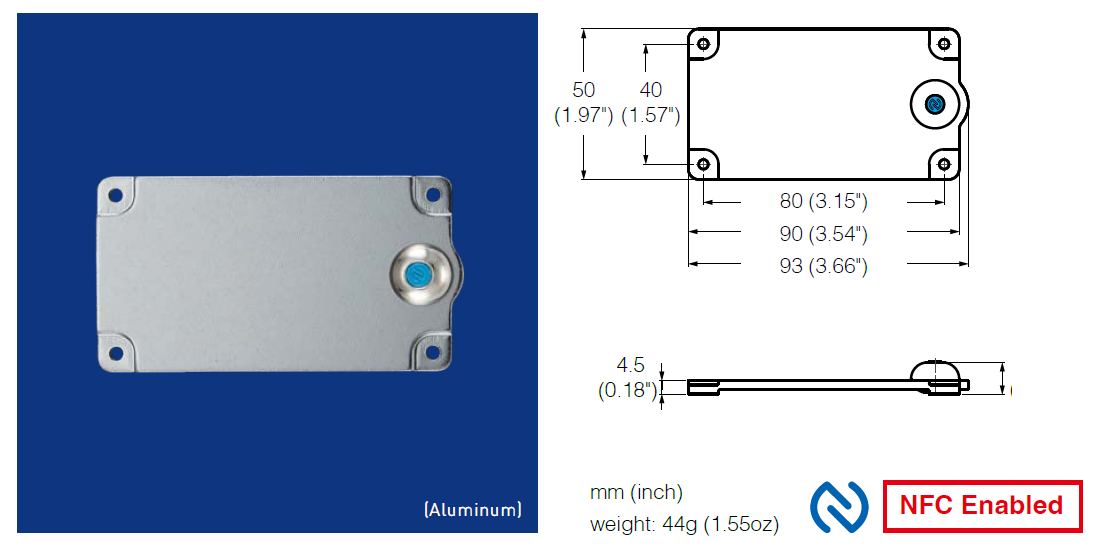
\includegraphics[width=\textwidth,keepaspectratio]{../../Images/Supra/SupraPlate.png}
%	\captionof{figure}{Maße der Suprapalte}
%	\label{fig:Supraplate}
%\end{center}

%In Abbildung \ref{Supraplate} ist ein flaches Aluminium-Gehäusebauteil dargestellt, in welches der NFC-Transponder integriert wurde. Dieses Bild zeigt detailliert die geometrischen Verhältnisse des Bauteils, das eine Gesamtlänge von 93 mm (3,66") und eine Breite von 50 mm (1.97") aufweist. Der Abstand zwischen den Montagebohrungen ist mit 80 mm in der Länge und 40 mm in der Breite bemaßt.
%
%In der Seitenansicht ist zu sehen, dass die Grundplatte eine Materialstärke von 4,5 mm (0.18") besitzt, während die Erhebung für den integrierten Chip die Gesamthöhe lokal begrenzt steigert. Gemäß der technischen Zeichnung beträgt das Gesamtgewicht dieser Aluminium-Komponente 44 g (1,55 oz). Die Abbildung verdeutlicht zudem die Positionierung des Transponders an der Stirnseite, um eine optimale Erreichbarkeit für NFC-Lesegeräte zu gewährleisten.

%Nachfolgende Tabelle (	) zeigt die im Datenblatt %\cite{} entnommen technischen Eigenschaften des Supra 228.

%
%\begin{table}[h!]
%	\caption{Supra 228} %\cite{}
%	\begin{center}
%		\begin{tabular}{|l|l|}
%			\hline
%			\textbf{Parameter} &\textbf{Detail} \\
%			\hline
%			Funktionalität &  	\\
%			\hline
%			RF Protokoll & ISO 15693 	\\
%			\hline
%			Betriebsfrequenz & 13,56MHz 	\\	
%			\hline
%			Speicherkonfiguration  & UID 16 Bit, Benutzerdaten 2 KB 	\\	
%			\hline
%			Lese-/Schreibfähigkeit & Lesen / Schreiben  	\\	
%			\hline
%			Leistung &   	\\	
%			\hline
%			Lesereichweite & max. 5mm 	\\	
%			\hline
%			Ausrichtung  & Lesung von der Vorderseite \\	
%			\hline
%			IP-Schutzklasse & IP68 \\	
%			\hline
%			Physikalische Eigenschaften &   \\	
%			\hline
%			Werkstoffe & PA 6 + 30 GF, Aluminium (eloxiert) \\	
%			\hline
%			Befestigungssystem & Universell einsetzbar \\
%			\hline
%			Farbe Tag & Türkisblau 	\\	
%			\hline
%			Farbe Gehäuse & Poliert 	\\	
%			\hline
%			Betrieb &  	\\	
%			\hline
%			Maximale Umgebungstemperatur & 125 °C / 257 °F 	\\	
%			\hline
%			Minimale Betriebstemperatur & -30 °C / -22 °F	\\	
%			\hline
%			Maximale Dauerbetriebstemperatur  & 125 °C / 257 °F 	\\	
%			\hline
%			Minimale Dauerbetriebstemperatur & -30 °C / -22 °F	\\	
%			\hline
%			Wasser- und eisbeständig & Ja \\	
%			\hline
%		\end{tabular}
%		\label{XXXXXXXXXXXXXXXXXXXXX}
%	\end{center}
%\end{table} 




\subsection{Merkmale}
\begin{itemize}{
\item UNC-Gewinde 
\item NFC-fähiges Mobilgerät oder Smartphone
	(iOS 14 oder höher erforderlich / Android 12 oder höher erforderlich) kann als Lesegerät verwendet werden.
\item Korrosionsbeständiger Edelstahl. 
\item Erfüllt die Anforderungen des US-Militärstandards MIL-STD-810H.
\item Erfüllt die Stoßfestigkeitsklasse IK10.
\item Erfüllt die höchste Schutzklasse IP68 für Staub- und Wasserdichtigkeit.
\item Einzigartiges Design der proprietären Wafer-Antennen-Chip-Konstruktion.
\item Patente in mehreren Ländern.
\item Durch die Verwendung der Supra Digital Chips in Verbindung mit einer Asset-Management-Anwendung eines Drittanbieters lassen sich Produktrückverfolgbarkeit, Herstellerauthentifizierung und digitalisierte Produktinformationen realisieren.
\item Patent in mehreren Ländern

} \end{itemize}

\begin{center}
	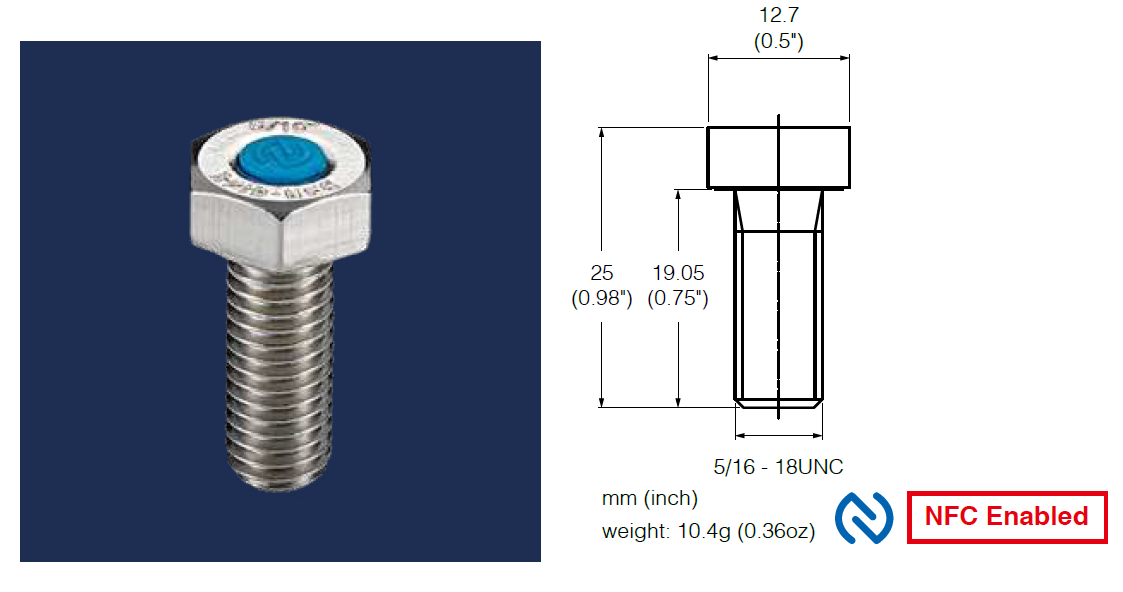
\includegraphics[width=\textwidth]{../../Images/Supra/SupraBolt.png}
	\captionof{figure}{Maße Des SupraBolt`s}
	\label{fig:NFCScrew}
\end{center}
In Abbildung \ref{NFCScrew} ist die technische Zeichnung sowie eine perspektivische Ansicht des Bauteils dargestellt. Das Bild zeigt einen Sechskantschraubbolzen mit den Abmessungen 25mm (0,98") in der Gesamtlänge und einer Schaftlänge von 19,05mm (0,75").Dieses Bild verdeutlicht zudem die Kopfgeometrie, welche einen Durchmesser von 12,7mm (0,5") aufweist. Aus der Darstellung geht hervor, dass das Bauteil mit einem 5/16 - 18UNC Gewinde versehen ist. Hinsichtlich der Massenbilanz ist in der Abbildung ein Gesamtgewicht von 10,4 g (0,36oz) spezifiziert.

Nachfolgende Tabelle (	) zeigt die im Datenblatt %\cite{} entnommen technischen Eigenschaften des Supra 228.

\begin{table}[h!]
	\caption{SupraBolt} %\cite{}
	\begin{center}
		\begin{tabular}{|l|l|}
			\hline
			\textbf{Parameter} &\textbf{Detail} \\
			\hline
			Funktionalität &  	\\
			\hline
			RF Protokoll & ISO 15693 	\\
			\hline
			Betriebsfrequenz & 13,56MHz 	\\	
			\hline
			Speicherkonfiguration  & UID 16 Bit, Benutzerdaten 2 KB 	\\	
			\hline
			Lese-/Schreibfähigkeit & Lesen / Schreiben  	\\	
			\hline
			Leistung &   	\\	
			\hline
			Lesereichweite & max. 5mm 	\\	
			\hline
			Ausrichtung  & Lesung von der Vorderseite \\	
			\hline
			IP-Schutzklasse & IP68 \\	
			\hline
			Physikalische Eigenschaften &   \\	
			\hline
			Werkstoffe & PA 6 + 30 GF, Edelstahl \\	
			\hline
			Befestigungssystem & Universell einsetzbar \\
			\hline
			Farbe Tag & Türkisblau 	\\	
			\hline
			Farbe Gehäuse & Poliert 	\\	
			\hline
			Betrieb &  	\\	
			\hline
			Maximale Umgebungstemperatur & 125 °C / 257 °F 	\\	
			\hline
			Minimale Betriebstemperatur & -30 °C / -22 °F	\\	
			\hline
			Maximale Dauerbetriebstemperatur  & 125 °C / 257 °F 	\\	
			\hline
			Minimale Dauerbetriebstemperatur & -30 °C / -22 °F	\\	
			\hline
			Wasser- und eisbeständig & Ja \\	
			\hline
			\end{tabular}
		\label{XXXXXXXXXXXXXXXXXXXXX}
	\end{center}
\end{table} 

\subsection{Patent}
\begin{itemize}{
		\item Deutsches Patent:		602018032891.2
		\item Taiwan Patent: 		M573545
		\item Taiwan-Patent:		I638765
		\item China-Patent:			ZL 201821589819.6
		\item China-Patent:			ZL 2017 1 0821524.0
		\item Japan-Patent:			3219858
		\item Japan-Patent:			3220091
		\item US-Patent:			10607128
		\item US-Patent:			10235617
		\item US-Patent:			11305844
		\item Italienisches Patent:	3627396
		\item Britisches Patent:	3627396
		
}\end{itemize}

%\section{Der MIL STD 810}
%
%\subsection{Was ist MIL STD 810?}
%
%Der MIL STD 810 ist ein Standard aus dem US-Militär. Die Norm spezifiziert die Umwelt-Testbedingungen, welche militärische Geräte unbeschädigt aushalten müssen, wie z.B. Regenwasser, Luftfeuchtigkeit, Schock, Vibration, Staub und Schimmelbefall. Hersteller von militärischer Ausrüstung führen diese Tests durch, um die Einhaltung des Standards zu demonstrieren. %\cite{}https://heinen-elektronik.de/glossar/mil-std-810/#was-ist-mil-std-810
%
%\subsection{Welche Aussagekraft hat MIL STD 810?}
%
%Die Bedeutung von MIL STD 810 liegt in seiner Rolle als Maßstab für die Haltbarkeit und Zuverlässigkeit von Ausrüstung unter extremen Bedingungen. Obwohl die Einhaltung des Standards nicht garantiert, dass ein Gerät allen aufgeführten Bedingungen getestet wurde, bietet sie eine wichtige Orientierungshilfe für Hersteller und Abnehmer. Für genauere Informationen über die Beständigkeit eines spezifischen Geräts wird auf die angegebene IP-Schutzart verwiesen.
%%\cite{}https://heinen-elektronik.de/glossar/mil-std-810/#was-ist-mil-std-810




%
%\subsection{Beschreibung Supraplate}
%Digitale Typenschilder stellen eine bahnbrechende Lösung dar, die sowohl in den Vereinigten Staaten als auch in der Europäischen Union die Einhaltung gesetzlicher Vorschriften gewährleistet und
%die Verwaltung durch IoT-Technologie verbessert.
%In der EU schreiben Richtlinien wie die Maschinenrichtlinie und die Arbeitsmittelrichtlinie eine eindeutige
%Kennzeichnung von Geräten und Sicherheitsbeschilderung vor. Digitale Typenschilder vereinfachen die Einhaltung der Vorschriften, indem sie wichtige Informationen wie Herstellerangaben,
%Modellnummern und CE-Kennzeichnungen digital anzeigen und
%so für eine Sichtbarkeit und Klarheit sorgen, die den EU-Standards entsprechen.
%In ähnlicher Weise verlangen die OSHA-Vorschriften in den USA eine wirksame Sicherheitskennzeichnung und Gefahrenkommunikation.
%Digitale Typenschilder erfüllen nicht nur diese Anforderungen, sondern ermöglichen auch Echtzeit-Aktualisierungen und Fernüberwachung
%über IoT-Konnektivität. Dies stellt sicher, dass Sicherheitsinformationen aktuell und zugänglich bleiben, was die Sicherheit am Arbeitsplatz und die Einhaltung von Vorschriften verbessert.
%Durch den Einsatz von IoT-Technologie bieten digitale Typenschilder Vorteile, die über herkömmliche statische Etiketten hinausgehen. Sie
%bieten dynamische Verwaltungsfunktionen und ermöglichen proaktive Wartungswarnungen, Ferndiagnosen
%sowie die Überwachung der Einhaltung von Vorschriften. Dieser digitale Ansatz vereinfacht nicht nur die Einhaltung
%gesetzlicher Vorschriften, sondern verbessert auch die betriebliche Effizienz und Sicherheit sowohl in den USA als auch in der EU.
%Zusammenfassend stellen digitale Typenschilder einen entscheidenden Fortschritt bei der Einhaltung gesetzlicher Vorschriften und
%im Management dar, da sie sich nahtlos an US-amerikanische und EU-Standards anpassen und gleichzeitig die Möglichkeiten des IoT
